\section{Plan de proyecto}

\subsection{Etapas e Iteraciones}

El desarrollo del proyecto se elaborar\'a en cuatro etapas: Incepción, Elaboración, Construcción y Transferencia. Durante la etapa de incepción se terminar\'an de consolidar los requerimientos funcionales y atributos de calidad de manera que queden definidos los drivers de la arquitectura. En la etapa de elaboración se elaborar\'a la especificación y modelos necesarios para comprender el funcionamiento del sistema. Durante la etapa de construcción se implementan los m\'odulos especificados y en la etapa de transferencia se procede a realizar el \textit{deployment} de las distintas piezas del sistema.  
\\ \par

La primera iteración de la etapa de elaboración consistirá en realizar la interfaz de los usuarios, ya que permitirá tener documentado en una etapa temprana todos los requisitos que se deber\'an cumplir para que el usuario pueda registrar los votos. Otra ventaja de tomar esta tarea en una etapa preliminar es la capacidad de poder usar la interfaz para mostrar al cliente como está funcionando el sistema (es decir, hay algo concreto a mostrar a medida que se van agregando funcionalidades), además de que permite un mayor grado de confiablidad para el testing de usabilidad. 
\\ \par
Cada iteración está dividida en varias etapas. Lo dividimos en varios m\'odulos que consideramos que agrupan todas las funcionalidades que deber\'a tener la interfaz, estas son: el m\'odulo de autenticación, el m\'odulo de envio de votos, el m\'odulo de formulario de votaci\'on y una \'ultima fase que testea la integraci\'on de los m\'odulos y corrige los errores correspondientes.

% La primera iteración comprenderá principalmente tareas de gestión y capacitación de los desarrolladores. Se tomó esta decisión porque identificamos varios intereses en conflicto y consideramos que es necesario establecer una prioridad entre ellos tan tempranamente como sea posible. Para hacer esto correctamente será necesario en primer lugar capacitar al equipo de desarrollo y de comunicación con los stakeholders en temas de seguridad. Priorizamos este tema en particular por haber sido considerado un atributo de calidad prioritario en el QAW y por la falta de capacitación del equipo en el mismo. 
%Una vez realizada la capacitación será necesario identificar arquitecturas alternativas priorizando de manera diferente los distintos intereses en conflicto.
%\\ \par
%Contando con distintas alternativas arquitectónicas se realizará una serie de reuniones con los distintos stakeholders informándoles por qué los distintos intereses entran en conflicto desde un punto de vista tecnológico y en qué medida beneficia cada posible decisión arquitectónica a concretar un objetivo u otro.
%\\ \par
%Es crucial que la totalidad del equipo tenga conocimientos suficientes de seguridad para garantizar que no sean introducidas vulnerabilidades en módulos aparentemente no relacionados con el tema, por lo que la capacitación de los desarrolladores continuará y se solapará con las reuniones con los stakeholders. 

\subsubsection{Gantt}

%% El primer Gantt tiene que tener todos los casos de uso, el segundo muestra todas las etapas de una iteracion, incluyendo disenio, impmentacion, testing
Algunas aclaraciones generales: para elaborar los diagramas contamos con un equipo de cuatro personas, un l\'ider de proyecto, un diseñador de arquitecturas de software, un programador, y un tester. Una limitaci\'on del programa que utilizamos para realizar los diagramas es que dos tareas pueden ser asignadas a una misma persona sin chequear que la persona pueda satisfacer las dos tareas, por lo que creamos algunas dependencias ficticias para mostrar que la tareas no pueden ser realizadas al mismo tiempo. Otra consecuencia de esto es que tambi\'en hay tareas que pueden estar solapadas y no se ven (especialmente en la vista general).

\par

En el primer diagrama mostramos cómo planeamos el proyecto a nivel general viendo así las distintas etapas y teniendo un tiempo estimado para las entregas. Agregamos tambi\'en tareas relacionadas con la administración del proyecto tal como la licitaci\'on de los servicios que utilizará el sistema y la capacitación del equipo de desarrollo. En el diagrama se muestra colapsadas las tareas realacionadas con la Interfaz del Usuario puesto que lo mostraremos en detalle más adelante. Si bien en el diagrama los productos parecen que depeden entre si, esto se debe al trabajo de este equipo, podrían existir módulos realizandose en paralelo. El orden en el que se realizan los productos es el que creemos que logra mejor como mostrar los avances del producto. El tiempo estimado para finalizar el desarrollo son 132 dias (aproximadamente 26 semanas).	

\par
\begin{figure}[H]
\begin{center}
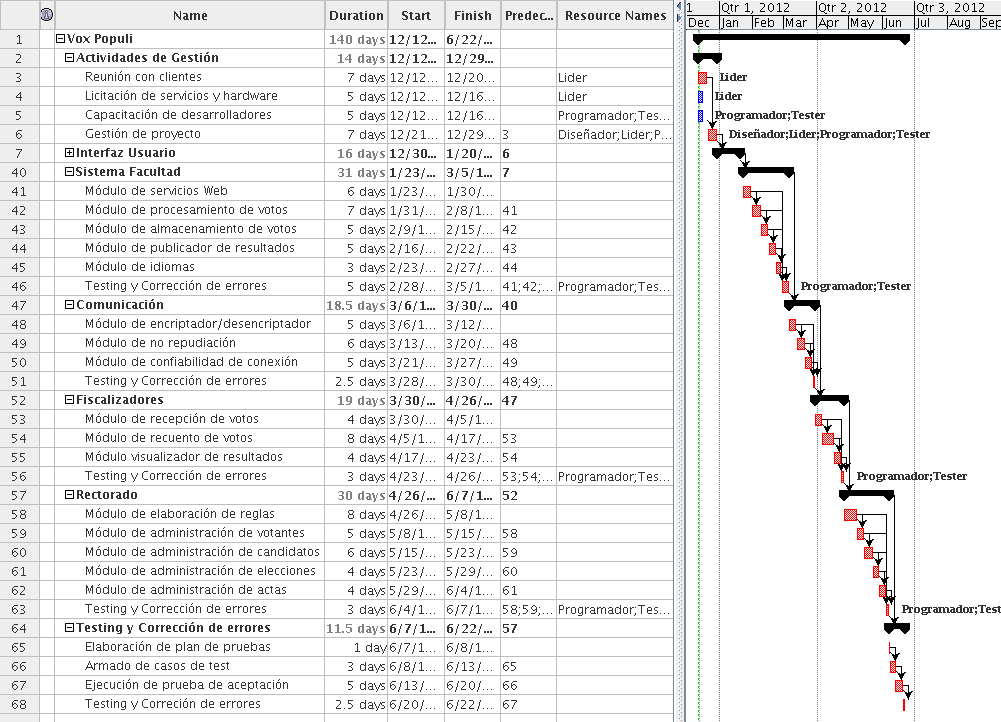
\includegraphics[scale=0.6]{./imagenes/gantintegral.png}
\end{center}
\end{figure}

\par
En un segundo diagrama hicimos un zoom sobre la primera iteración de la primera etapa de elaboración, que tal como habíamos dicho corresponde a la interfaz del usuario. Dividimos la interfaz de usuario en los m\'odulos dichos anteriormente. A cada uno de los m\'odulos les asignamos tareas a realizarce, cada uno contendrá tareas similares: una tarea de an\'alisis funcional, una tarea de diseño, una tarea de implementaci\'on, una tarea de testing y una tarea de correcci\'on de errores.

\par
\begin{figure}[H]
\begin{center}
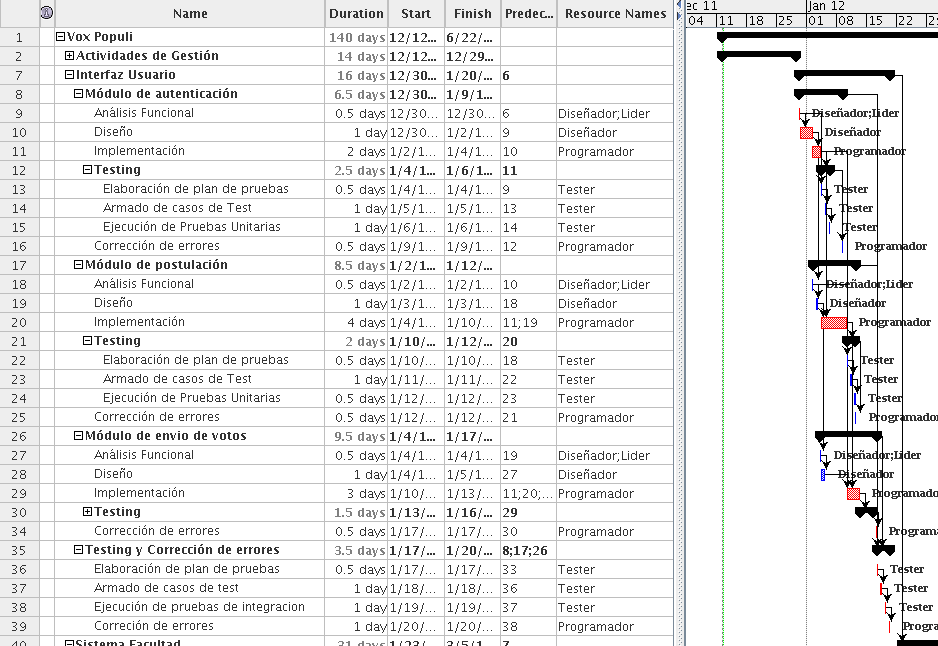
\includegraphics[scale=0.6]{./imagenes/gantiteracion.png}
\end{center}
\end{figure}

% \renewcommand{\labelitemi}{$\tiny \blacksquare$}

%Algunos puntos a destacar del diagrama:
%\begin{itemize}
% \item Podemos ver que en esta iteración el equipo de desarrollo realizará dos tareas. Durante la primera semana, la capacitación que consiste en instruir al equipo en diversos temas relacionados con seguridad ya que queremos minimizar problemas de este tipo. Durante la segunda semana pueden comenzar tareas de desarrollo con los m\'odulos relacionados a comunicación, ya que se encuentra aislado al resto del sistema y tienen partes que no requieren de una arquitectura definida.
% \item El equipo de diseñadores se encarga inicialmente de realizar una arquitectura preliminar, para empezar a analizar alguno de los riesgos y problemas que nuestra arquitectura deberá solucionar. Permite que se empiezen a analizar algunos de los problemas que se trataran con los stakeholders, y se ver\'an qu\'e elementos externos serán requeridos.
% \item Luego habr\'a una etapa de an\'alisis de mercado para estar informados de las distintas tecnologías foraneas con las que nuestro proyecto podr\'a contar. Un punto clave para el proyecto por ejemplo es hacer un an\'alisis de servidores y proveedores de internet, ya que debemos mantener una alta disponibilidad.
% \item Por último el equipo de diseñadores se encargará de reunirse con los stakeholders para terminar de definir la arquitectura. Para esto fue necesario tener una arquitectura preliminar, y haber investigado las tecnologías disponibles para consensuar aquellas a utilizar. 
%\end{itemize}
%\renewcommand{\labelitemi}{}


\subsection{Work Breakdown Structure} 

Utilizando la dinámica sugerida en las clases teóricas, generamos un WBS híbrido. En el primer nivel dividimos el sistema en 6 productos y procesos que capturan las distintas actividades a realizar para la construcción del sistema completo. Cada uno de los productos y procesos del primer nivel agrupan funcionalidades relacionadas, excepto Actividades de gestión, que se diferencia de los demás por relacionarse con el sistema en su totalidad.

Esta división no muestra todas las dependencias entre productos y procesos, muchas de las cuales terminarán de definirse en el diagrama de Gantt de la iteración que corresponda.
\\ \par

Los seis elementos del primer nivel serán: Interfaz, Sistema Facultad, Comunicación, Actividades de gestión, Fiscalizador y el Sistema Rectorado.
\\ \par
Interfaz comprende los productos y procesos relacionados con el relevamiento de requerimientos, casos de uso, codificación y prueba de la interfaz. Este producto seguramente podrá ser construído independientemente de los demás.
\\ \par
%TODO cambiar este parrafo que aplicaba para la primer entrega pero no ahora
Sistema Facultad incluye productos y procesos orientados a la construcción del sistema autónomo de cada Facultad, que se encargará de recibir y fiscalizar la totalidad de los votos correspondientes a la misma, además de distribuir información a los partidos políticos y el rectorado. Los requerimientos funcionales y atributos de calidad prioritarios definitivos para este producto dependerán de varias tareas de gestión a realizarse en las primeras iteraciones, con el fin de consensuar soluciones de compromiso a los diversos intereses, que actualmente se encuentran en conflicto, como ser la posibilidad de contar con resultados parciales y un registro de votantes en tiempo real, en contraposición con la idea de garantizar el voto secreto.
\\ \par
%TODO lo mismo que antes
Comunicación está conformado por productos y procesos proveedores de comunicación entre los distintos sistemas de cada Facultad. Este producto, tal como Sistema Facultad, depende de la definición de varios aspectos de los atributos de calidad y requerimientos funcionales, por lo que dependerá de los procesos de actividades de gestión.
\\ \par
%TODO lo mismo que antes
Actividades de gestión reúne diversos procesos que pueden ser separados en unos pocos ejes. En primer lugar está la capacitación de los stakeholders, explicando por qué los intereses expresados entran en conflicto y cuáles alternativas arquitectónicas permiten priorizar uno u otro y en qué medida.
En segundo lugar habrán gran cantidad de procesos destinados a la validación intermedia del avance de la construcción del sistema, que consistirá en reuniones pequeñas con los principales interesados y algunas reuniones más grandes donde se muestren funcionalidades de interes general.
También habrán actividades de planificación en general, que comprenderá, por ejemplo, la confección de los diagramas de Gantt de cada iteración.
Por último será necesario capacitar al equipo en temas de seguridad, para lograr que sea tenida en cuenta en todos los niveles de desarrollo y elicitación de requerimientos. Esta capacitación será una de las primeras actividades a realizarse.
\\ \par
%TODO fiscalizador se refiere a los componentes que constituyen la agrupacion politica
Fiscalizador es el producto que tendran los diversos partidos politicos. Nuestro sistema deberá armar estos sub sistemas que permitiran que los partidos políticos se comuniquen con las facultades que deseen y además se realize el recuento de votos en forma local de manera que se logre una elección más transparente. 
\\ \par
Sistema Rectorado incluye los productos que el rectorado estaba interesado en tener para realizar diversas tareas de gestión. Una de esas tareas era tener conocimiento de los usarios que ya votaron en la elección. Además el rectorado solicitó que el sistema permita cambiar su funcionalidad para realizar plebiscitos, por lo que agregamos la funcionalidad de definir las reglas de las elecciones permitiendo que sea facilmente modificables. También tiene la posiblidad de resolver los conflictos para los resultados de una elección y aceptar un acta que fue generada por el sistema. Por último puede administrar elecciones, decidir su fecha de inicio y fecha de fin.

\begin{itemize}
 \item {\bf \emph{WBS Vox}}
\begin{itemize}
 \item {\bf Sistema Facultad}
\begin{itemize}
 \item \emph{M\'odulo de servicios Web} 
\begin{itemize}
 \item Se encarga de la comunicación con las distintas interfaces web.
\end{itemize}
 \item \emph{M\'odulo de procesamiento de votos} 
\begin{itemize}
 \item Se encarga de recibir los votos y procesarlos según las reglas enviadas por el decanato.
\end{itemize}
 \item \emph{M\'odulo de almacenamiento de votos} 
\begin{itemize}
 \item Se encarga registrar los votos junto con las personas que votaron, publicarlos y archivar.
\end{itemize}
 \item \emph{M\'odulo de publicador de resultados} 
\begin{itemize}
 \item Se encarga de enviar al rectorado la información de una elección.
\end{itemize}
 \item \emph{M\'odulo de idiomas}
\begin{itemize}
 \item Se encarga de adminisitrar los idiomas soportados en la interfaz de usuario
 \item {\bf Caso de uso:} Cambio de idioma en la interfaz de usuario
\end{itemize}
\end{itemize}
 \item {\bf Interfaz de Usuario}
\begin{itemize}
 \item \emph{M\'odulo de autenticación}
\begin{itemize}
 \item Se encarga de validar que el usuario es miembro del departamento
 \item {\bf Caso de uso:} Generando contrase\~na
 \item {\bf Caso de uso:} Ingresando al sistema
\end{itemize}
 \item \emph{M\'odulo de envio de votos}
\begin{itemize}
 \item Se encarga de enviar el voto al sistema de la facultad
 \item {\bf Caso de uso:} Emitiendo un voto
\end{itemize}
 \item \emph{M\'odulo de postulación}
\begin{itemize}
 \item Se encarga de postularse para una elección
 \item {\bf Caso de uso:} Postulandose para las elecciones
\end{itemize}
\end{itemize}
 \item {\bf Comunicación}
\begin{itemize}
 \item \emph{M\'odulo de encriptación/desencriptación}
\begin{itemize}
 \item Se encarga de encriptar y desencriptar la información enviada y recibida
 \item {\bf Caso de uso:} Conexión desde diversas plataformas
\end{itemize}
 \item \emph{M\'odulo de no repudiación}
\begin{itemize}
 \item Se encarga de verificar que las entidades que pretenden ser miembros del departamento realmente lo sean
\end{itemize}
 \item \emph{M\'odulo de confiabilidad de conexión}
\begin{itemize}
 \item Se encarga de controlar los canales que deben ser confiables
\end{itemize}
\end{itemize}
 \item {\bf Actividades de Gestión}
\begin{itemize}
 \item \emph{Capacitación de desarrolladores}
\begin{itemize}
 \item Se debe capacitar a los desarrolladores para que sistema implentado sea seguro
\end{itemize}
 \item \emph{Licitación de servicios y hardware}
\begin{itemize}
 \item Se debe hacer un analisis del hardware a ser utilizado y servicios externos que se utilizaran
\end{itemize}
 \item \emph{Armado de plan de proyecto}
\begin{itemize}
 \item Se debe realizar tareas de gestión relacionadas con la planificación
\end{itemize}
\end{itemize}
 \item {\bf Fiscalizadores}
\begin{itemize}
 \item \emph{M\'odulo de recepción de votos}
\begin{itemize}
 \item Se encarga de subscripción y recepción de los votos del sistema de la facultad
\end{itemize}
 \item \emph{M\'odulo visualizador de resultados}
\begin{itemize}
 \item Se encarga, para una elección, mostrar los canidatos que votaron y los resultados en caso de ser posible
 \item {\bf Caso de uso:} Viendo resultados
\end{itemize}
 \item \emph{M\'odulo de recuento de votos}
\begin{itemize}
 \item Se encarga de procesar los votos que recibe haciendo un recuento de votos
 \item {\bf Caso de uso:} Fiscalizando votaci\'on
\end{itemize}
\end{itemize}
 \item {\bf Sistema Rectorado}
\begin{itemize}
 \item \emph{M\'odulo de confección de reglas}
\begin{itemize}
 \item Se encarga de definir reglas para procesar los votos
 \item {\bf Caso de uso:} Reglamentando elecciones
\end{itemize}
 \item \emph{M\'odulo control de votantes}
\begin{itemize}
 \item Se encarga de consultar a los sistemas de las facultades quienes votaron
 \item {\bf Caso de uso:} Auditando votantes
\end{itemize}
 \item \emph{M\'odulo de administración de candidatos}
\begin{itemize}
 \item Se encarga de administrar a los candidatos de las distintas facultades
\end{itemize}
 \item \emph{M\'odulo de administración de elecciones}
\begin{itemize}
 \item Se encarga de administrar el comienzo y la finalización de las elecciones
 \item {\bf Caso de uso:} Agregando elección
 \item {\bf Caso de uso:} Modificando elección
\end{itemize}
 \item \emph{M\'odulo de administración de actas}
\begin{itemize}
 \item Se encarga de arreglar conflictos y aceptar actas
 \item {\bf Caso de uso:} Resolviendo conflictos
 \item {\bf Caso de uso:} Aceptando acta
\end{itemize}
\end{itemize}
\end{itemize}
\end{itemize}


Para la facilitación de la lectura omitimos escribir el nivel más bajo del WBS para poder ver descripciones de cada m\'odulo. Cada uno de los m\'odulos pueden ser divididos en diferentes procesos,
los cuales serán asignados dependiendo del producto.
\begin{itemize}
 \item Analisis funcional
 \item Diseño
 \item Codificación
 \item Elaboración de Plan de Pruebas
 \item Ejecución de Pruebas Unitarias
 \item Ejecución de Pruebas de Integración
 \item Ejecución de Pruebas de Aceptación
 \item Correción de Errores
 \item Instalación en ambiente de prueba
 \item Verificación Final
 \item Revisión de Alcance
\end{itemize}	
